\documentclass[times, utf8, diplomski, numeric]{templates/template}
\usepackage{booktabs}

\begin{document}

\sveuciliste{SVEUČILIŠTE U ZAGREBU}
\fakultet{FAKULTET ELEKTROTEHNIKE I RAČUNARSTVA}

\title{Programska podrška sustava za određivanje i upravljanje orijentacijom satelita}

\thesisnumber{2346}

\author{Ivan Vnučec}

\maketitle

% Ispis stranice s napomenom o umetanju izvornika rada. 
\izvornik

% TODO: Dodaj zahvalu
\zahvala{Ovdje ide zahvala}

\tableofcontents

% TODO: delete me
\nocite{*}

\chapter{Uvod}{
    \section{Mali sateliti}{
        %- sto su mali sateliti
        Mali sateliti su skupina satelita koji su, u usporedbi sa konvencionalnim satelitima, uvelike ograničeni prema masi, cijeni, kao i prema vremenu potrebnom da ih se razvije. Sve je to izravan rezultat revolucije u elektronici i računarstvu.\cite{hrvatskiVojnik}.

        %- tko ih koristi
        Primjene malih satelita nalazimo u svim granama svemirske industrije: u telekomunikaciji, navigaciji, opservaciji Zemlje, znanstvenim istraživanjima i dr.
        
        %- zasto ih koristimo
        Njihova zastupljenost na tržištu raste iz godine u godinu jer pružaju jeftin i brz razvoj uz relativno male tehničke zahtjeve \cite{rastMalihSatelita}. Primjenom većeg broja malih satelita povezanih u konstelaciju, moguće je primjerice pokriti veću površinu zemlje i tako stvoriti uvijek dostupni internet ili navigacijski sustav.
        
        \subsection{Podjela}{
            Iako postoje više vrsta podjela satelita u ovisnosti od izvora do izvora, navest ćemo podjelu prema FAA \engl{Federal Aviation Administration} koja uključuje satelite sa najvećom, pa sve do satelita sa najmanjom masom \cite{podjelaPremaMasi}. Podjelu je moguće vidjeti u tablici \ref{tbl:podjelaSatelita}.

            \begin{table}[htb]
            \caption{Podjela malih satelita prema masi}
            \label{tbl:podjelaSatelita}
            \centering
            \begin{tabular}{ll} \toprule
            Naziv kategorije satelita & Masa (kg) \\ \midrule
            Small & 601 - 1200 \\
            Mini & 201 - 600 \\
            Micro & 11 - 200 \\
            Nano & 1.1 - 10 \\
            Pico & 0.09 - 1 \\
            Femto & 0.01 - 0.1 \\ \bottomrule
            \end{tabular}
            \end{table}

            Maleni sateliti \engl{Small} teže manje od 1200 kilograma, cijena im je nešto manje od 30 milijuna GBP (britanskih funti) za izradu i lansiranje te je potrebno od 2 do 3 godine za njihov razvoj. Mini sateliti teže do 600 kilograma i njihov razvoj traje dvije godine po cijeni do 30 milijuna GBP. Micro sateliti su teški manje od 200 kilograma i koštaju manje od 10 milijuna GBP. Ispod te klase nalaze se Nano sateliti, težine do 10 kilograma, te Pico i Femto sateliti težine manje od 1 kilograma \cite{hrvatskiVojnik}.

            \subsubsection{Cubesat format}{
                %- sto je cubesat satelit
                %- od cega se sastoji, 
                %    - građa, 
                %    - nacin slaganja dodatnih modula
                %- kojih sve verzije cubesat satelita postoje
                %- zasto bas kocka
                %- prednosti i mane cubesat satelita
                %- navesti negdje brojke o udijelu cubesat sateltia u ostalim satelitima kroz godine
                %- zasto je popularan cubesat format
            }
        }
        
        \subsection{Metode lansiranja}{
            %- objasniti kako se sateliti lansiraju
            %    - objasni da oni nisu glavni payload
            %    - objasni kako su pakirani
            %    - objasni u koje orbite mogu ici
            %    - objasni tvrtke koje se bave lansiranjem
            %- navedi koliko najcesce kosta lansiranje
            %- navedi kako najlakse iznajmit lansiranje
            %- rast lansiranja nanosateltia iz godine u godinu
            %    - pronaci negdje neke brojke o lansiranju cubesat satelita po godinama
        }
        
        \subsection{Povijesni pregled misija}{
            %- navesti neke komercijalne primjene do sada
            %- navesti znanstvene misije do sada
        }
    }

    \section{Korisni teret satelita}{
        % sto je korisni teret satelita
        Korisni teret satelita \engl{payload} jest podsustav, ili skupina podsustava, koji imaju za cilj ispuniti zadaću koja im je dodijeljena (misija). Primjerice, ako je cilj satelita fotografiranje Zemljine površine, onda će njegov koristan teret biti sustav za fotografiranje (kamera). Ili primjerice ako želimo uspostaviti komunikaciju sa satelitom, što je gotovo uvijek slučaj, onda će njegov korisni sustav biti sustav za komunikaciju.

        \subsection{Vrste tereta}{
            %- navesti korisne terete koje satelit ima u ovisnosti o tipu misije
            Ovisno o tipu misije, razlikujemo podsustave koje je moguće svrstati u nekoliko sljedećih kategorija:

            \begin{itemize}
                \item Opservacija Zemlje
                \item Komunikacija
                \item Navigacija
                \item Znanost i tehnologija
            \end{itemize}

            Sustavi za opservaciju Zemlje sadrže uređaje koji promatraju Zemljinu površinu ili atmosferu. Najčešće takav sustav sadrži kameru koja fotografira u odabranom dijelu spektra. Zbog toga što na takvom sustavu osim kamere imamo i objektive koji omogućuju velika uvećanja, potrebno je da posjedujemo mogućnost preciznog usmjeravanja kamere. Također, sustav za komunikaciju, osim sklopovlja za obradu signala, sadrži i antene. Kako bi pospješili prijem i odašiljanje, potrebno je usmjeriti antenu prema drugoj anteni na Zemlji \cite{sattelitePayload}.

            \subsection{Važnost kontrolirane orijentacije}{
                \subsubsection{Detumbling}{
                    Osim gore opisanih sustava kojima je važna kontrola orijentacije, navest ćemo još jedan primjer gdje nam je kontrola orijentacije važna. Naime, prilikom izbacivanja satelita iz samog prijevoznog sredstva u svemir, događa se nekontrolirana rotacija satelita. Kako bi satelit zaustavio rotaciju, aktivni sustav za determinaciju i kontrolu orijentacije \engl{Attitude Control and Determination System - ADCS} ulazi u posebni način rada \engl{detumbling} u kojem će zaustaviti nekontroliranu rotaciju. Takav zahvat može potrajati tjednima ili mjesecima, ovisno o tipu satelita \cite{fersat}.
                }

                \subsubsection{Ukratko o ADCS sustavu}{
                    ADCS sustav određuje orijentaciju pomoću podataka iz senzora. Senzori najčešće ne daju direktno vrijednost orijentacije već se orijentacija estimira pomoću estimacijskih algoritama. Problem senzora općenito je njihova neodređenost koja onda doprinosi da je estimacija orijentacije pogrešna. Zbog toga smo razvili estimacijske algoritme koje uzimaju grešku senzora u obzir te tako smanjuju neodređenost estimirane orijentacije.

                    Nakon što smo odredili orijentaciju, i ako ta orijentacija nije jednaka željenoj, slijedi postupak korekcije (kontrole). Postupak korekcije počinje računanjem razlike željene orijentacije i trenutno estimirane. Regulator orijentacije će pomoću te razlike orijentacije izračunati optimalnu korekciju koju je potrebno izvršiti kako bi došli u željenu orijentaciju. Korekciju orijentacije izvršavaju mehanički odnosno električni aktuatori. Aktuatori će stvoriti korekcijski moment koji satelit naposlijetku dovodi u željenu orijentaciju.
                }

                \subsubsection{Važnost ADCS sustava u radu satelita}{
                    Opisana estimacija i kontrola orijentacije ADCS sustava događa se u stvarnom vremenu kroz cijeli radni vijek satelita i ni u jednom trenu se ne smije dogoditi da satelit posjeduje neželjenu ili nekontroliranu orijentaciju jer to može značiti kraj misije.

                    NASA-ino istraživanje je pokazalo da je ADCS sustav zaslužan za 23\% grešaka na navigacijsko-kontrolnim sustavima \engl{Guidance, Navigation and Control - GN\&C}, i da je većina tih anomalija uzrokovala kraj misije \cite{greskeNaAdcsPostotak}. U nastavku ćemo navest jedan primjer greške na ADCS sustavu.

                    Lewis svemirska letjelica \cite{lewis} lansirana je 1997. godine s predviđenim radnim vijekom od 5 godina. Nakon postizanja uspješne orbite satelit je započeo sa normalnim radom i nije ga više bilo potrebno aktivno kontrolirati. U normalnom radu solarni paneli su bili upereni prema Suncu kako bi prikupili maksimalnu količinu energije. Zbog greške prilikom rada, jedan od aktuatora je stvarao konstantni moment oko jedne osi koju senzori nisu mogli prepoznati. Nakon nekoliko dana, satelit se je počeo nekontrolirano rotirat i solarni paneli nisu prikupljali dovoljno energije. Naposlijetku su inženjeri sa Zemlje uočili nekontroliranu orijentaciju ali je već bilo kasno jer se je baterija satelita potpuno ispraznila i komunikacija sa satelitom je bila zauvijek prekinuta \cite{greskeNaAdcsSlucajevi}.
                }
            }
        }
    }
}

\chapter{Osnovni kinematički model satelita}{
    Kako bi matematički prikazali rotacijsko gibanje satelita, satelit je prvo potrebno modelirati kao kruto tijelo. Mi ćemo u nastavku navesti samo osnovne izraze potrebne za modeliranje satelita, a potpune matematičke izraze i izvode moguće je pronaći u popratnoj literaturi \cite{adcsKnjiga}.

    \section{Osnovni parametri satelita}{
        Inercijska matrica \engl{Moment of inertia tensor} u pojednostavljenom smislu označava moment tromosti krutog tijela oko pojedine osi rotacije. Naglašavamo da je u pitanju pojednostavljena definicija i da ona nije strogo točna, no za naše potrebe je ona dovoljna. Inercijsku matricu predstavljamo kao:

        \begin{equation}
        \textbf{J} = 
        \begin{bmatrix}
            J_{xx} & J_{xy} & J_{xz} \\
            J_{yx} & J_{yy} & J_{yz} \\
            J_{zx} & J_{zy} & J_{zz}
        \end{bmatrix}
        .
        \end{equation}

        Moguće je pokazati da za svako kruto tijelo možemo pojednostaviti Inercijsku matricu te tako dobiti dijagonalnu inercijsku matricu. Takva matrica nam omogućuje izvedbu jednostavnijih izraza za rotaciju krutog tijela. Zbog nepotrebnog ulaženja u detalje kako je moguće dobiti dijagonalnu matricu, navest ćemo samo izraz kao:

        \begin{equation}
        \textbf{I} = 
        \begin{bmatrix}
            I_{xx} & 0      & 0 \\
            0      & I_{yy} & 0 \\
            0      & 0      & I_{zz} \\
        \end{bmatrix}
        .
        \end{equation}
    }

    \section{Eulerovi kutovi}{
        Eulerovi kutovi predstavljaju 3 kuta između nekog vektora i ortogonalnih osi koje razapinju Kartezijev koordinatni sustav. Ako želimo predstaviti rotaciju između jednog proizvoljnog vektora i nekog drugog vektora, onda to možemo napraviti na nekoliko načina. Jedan primjer takve rotacije navest ćemo u sljedećem primjeru:

        \begin{enumerate}
            \item Rotacija za kut $\psi$ oko orginalne z-osi \engl{yaw}.
            \item Rotacija za kut $\theta$ oko tranzicijske y-osi \engl{pitch}.
            \item Rotacija za kut $\phi$ oko transformirane x-osi \engl{roll}.
        \end{enumerate}

        Uzmemo li za primjer 3 uzastopne rotacije: prve oko orginalne z-osi, zatim druge oko tranzicijske y-osi i na kraju treće oko transformirane x-osi dobivamo rotaciju prikazanu na slici ispod: 

        \begin{figure}[htb]
        \centering
        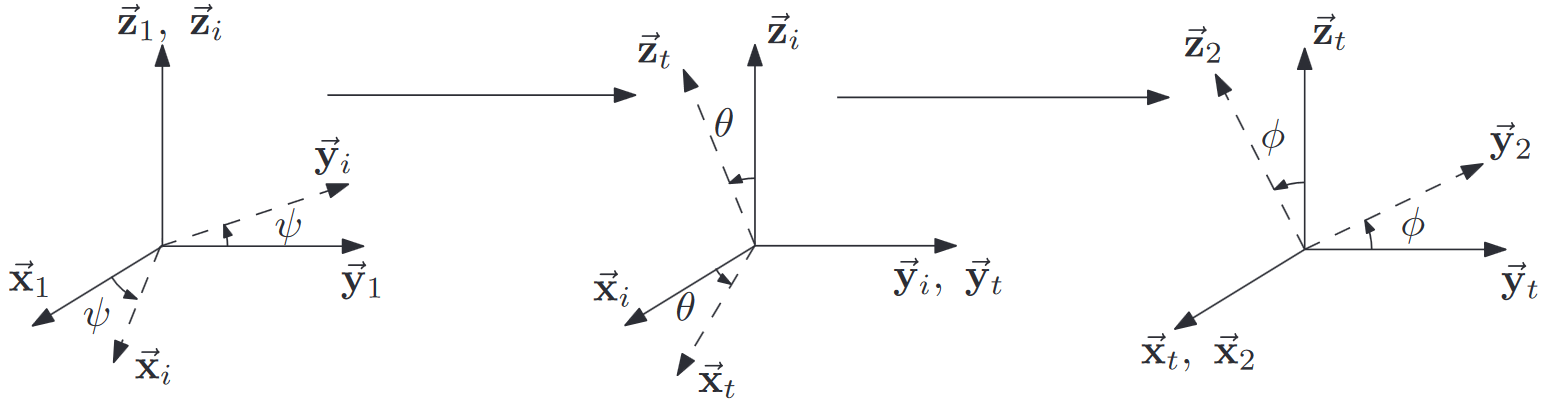
\includegraphics[width=1.0\textwidth]{images/eulerovi_kutovi.jpg}
        \caption{Tri uzastopne rotacije oko z-osi, y-osi i x-osi za kut $\psi$, $\theta$, i $\phi$}
        \label{fig:euler_rotacija}
        \end{figure}
    }

    \section{Kvaternioni}{
        - definicija kvaterniona
    }

    \section{Rotacijska matrica}{
        - definicija rotacijske matrice naslov 1.3.1

        \subsection{Prikaz pomoću Eulerovih kutova}{
            Takva sekvenca rotacija je jako česta u zrakoplovno-svemirskoj industriji i označava se kao 3-2-1 orijentacijska sekvenca \engl{attitude sequence}. Takvo ime je uzeto zato što je prva rotacija oko orginalne z-osi (oznaka 3), zatim slijedi rotacija oko tranzicijske y-osi (oznaka 2) te na kraju rotacija oko transformirane x-osi (oznaka 1).

            Matrica koja transformira jedan skup triju međusobno ortogonalnih vektora u drugi skup triju međusobno ortogonalnih vektora moguće je prikazati pomoću Eulerovih kutova kao:

            \begin{equation}
            \label{eq:euler_rot_mat}
            \begin{array}{rcl}
            \textbf{C}_{21}(\phi, \theta, \psi) & = & \textbf{C}_{x}(\phi) \textbf{C}_{y}(\theta) \textbf{C}_{z}(\psi) \\
            & = &
            \begin{bmatrix}
                c_{\theta}c_{\psi}                            & c_{\theta}s_{\psi}                            & -s_{\theta} \\
                s_{\phi}s_{\theta}c_{\psi} - c_{\phi}s_{\psi} & s_{\phi}s_{\theta}s_{\psi} + c_{\phi}c_{\psi} & s_{\phi}c_{\theta} \\
                c_{\phi}s_{\theta}c_{\psi} + s_{\phi}s_{\psi} & c_{\phi}s_{\theta}s_{\psi} - s_{\phi}c_{\psi} & c_{\phi}c_{\theta}
            \end{bmatrix}
            \end{array}
            ,
            \end{equation}

            gdje radi preglednosti vrijedi $s_{b}=\sin(b)$ i $c_{b}=\sin(b)$.

            Jedna mana reprezentacije rotacije pomoću Eulerovih kutova je tzv. singularnost. Može se pokazati da za svaku parametrizaciju rotacije može doći do singulariteta. Za naš primjer 3-2-1 sekvence singularitet nastaje kada je $\theta=\pm90^{\circ}$. Za takav slučaj rotacijska matrica postaje:

            \begin{equation}
            \textbf{C}_{21}(\phi, 90^{\circ}, \psi) =
            \begin{bmatrix}
                0                 & 0                  & -1 \\
                \sin(\phi - \psi) & \cos(\phi - \psi)  &  0 \\
                \cos(\phi - \psi) & -\sin(\phi - \psi) &  0
            \end{bmatrix}
            .
            \end{equation}

            Fizikalno, zbog singulariteta prva i treća rotacija unutar 3-2-1 sekvence se odvijaju oko jedne te iste osi. U tom slučaju roll i yaw ($\phi$ i $\psi$) su zapravo jednaki kutovi i ne mogu se jednoznačno odrediti. 

            Izvan singulariteta, moguće je jednoznačno odrediti sva tri Eulerova kuta. Ako rotacijsku matricu označimo kao:

            \begin{equation}
            \textbf{C} =
            \begin{bmatrix}
                c_{11} & c_{12} & c_{13} \\
                c_{21} & c_{22} & c_{23} \\
                c_{31} & c_{32} & c_{33} \\
            \end{bmatrix}
            ,
            \end{equation}

            iz jednadžbe \ref{eq:euler_rot_mat} moguće je dobiti Eulerove kutove kao:

            \begin{equation}
            \begin{array}{rcl}
                \phi   & = & \tan^{-1}(c_{23}/c_{33}),\\
                \theta & = & -\sin^{-1}(c_{13}),\\
                \psi   & = & \tan^{-1}(c_{12}/c_{11}).
            \end{array}
            \end{equation}

            \textbf{Naglašavamo kako je iznimno važno da prilikom definicije rotacije pomoću Eulerovih kutova naglasimo o kojoj sekvenci rotacije se radi (npr. 3-2-1) jer rotacijske sekvence ne komutiraju!}
        }

        \subsection{Prikaz pomoću kvaterniona}{
            %- TODO: nadji u knjizi
        }
    }

    \section{Rotacija}{
        \subsection{Prikaz pomoću Eulerovih kutova}{
            %- definicija rotacije preko eulerovih kuteva 1.59
        }

        \subsection{Prikaz pomoću kvaterniona}{
            %- TODO: nadji u knjizi
        }
    }

    \section{Jednadžba rotacijskog gibanja}{
        \subsection{Prikaz pomoću Eulerovih kutova}{
            %- cijelovita jednadzva rotacije cvrstog tijela 2.30
            %- pojednostavljene eulerove jednadzbe 2.42
        }

        \subsection{Prikaz pomoću kvaterniona}{
            %- TODO: nadji u knjizi
        }

        \section{Usporedba Eulerovih kutova i kvaterniona}{
            %- problemi neodredjenosti eulerovih kuteva
            %- prednost jednadzbi sa kvaternionima jer nema sin cos vec su algebarske
            %- mana sto na kraju krajeva nam je zgodno imati priakz u eulerovim
        }
    }
}

\chapter{Sustav za određivanje i upravljanje orijentacijom satelita (ADCS)}{
    \section{Uvod}{
        %- sto je sustav za određivanje i upravljanje orijentacijom satelita
        %    - navesti englesku skracenicu (koristi eng u latexu, vidi dokumentaciju pri dnu)
        %- koja je zadaca sustava za određivanje a koja sustava za upravljanje orijentacijom satelita
    }

    \section{Osnovni dijelovi}{
        \subsection{Računalo}{
            %- prikupljanje podataka
            %- obrada podataka
            %- kontrola orijentacije
            %- komunikacija
        }

        \subsection{Senzori}{
            %- koji sve postoje
            %- na kojem principima rade
            %- navesti neke tehnicke podatke svakog
            %- napraviti usporedbu između njih
            %    - cijena
            %    - preciznost
            %    - uvijeti rada
            %    - dostupnost
            %    - jednostavnost
            %    - potrosnja
        }

        \subsection{Aktuatori}{
            %- koji sve postoje
            %- na kojim principima rade
            %- tehnicki podatci
            %- usporedba između njih
            %    - cijena
            %    - preciznost
            %    - uvijeti rada
            %    - dostupnost
            %    - jednostavnost
            %    - potrosnja
        }
    }

    \section{Određivanje orijentacije}{
        \subsection{Korišteni senzori}{
            %- kako mjerimo kutnu brzinu
            %    - ziroskop
            %    - sto je ziroskop
            %    - problemi ziroskopa
        }

        \subsection{Algoritmi}{
            %- kako mozemo estimirati orijentaciju satelita
            %    - senzor fusion
            %    - navesti neke od algoritama
            %    - rekurzivni
            %    - ne rekurzivni
            %    - vidi s josipom jos neke koje je on razvijao
            %    - karla je jedan razvijala (stavi referencu)
        }
    }

    \section{Upravljanje orijentacijom}{
        \subsection{Korišteni aktuatori}{
            %- navesti aktuatore
            %- zamasnjake, magnetorqere
            %- navesti problem zasicenja zamasnjaka
        }

        \subsection{Algoritmi}{
            %- ukratko o upravljanju orijentacijom
            %- ukratko o upravljanju kutnom brzinom
            %- regulacija
            %    - navesti PID regulator kao regulator
            %    - opisati sto je PID regulator
            %    - navesti quaternion regulator kao regulator
            %        - jednadzbe
            %        - dodaj referencu na paper
        }
    }

    \section{Sklopovlje}{
        \subsection{Tiskana pločica}{
            %- ukratko o razvijenoj plocici
            %- staviti kakvu shemu
        }

        \subsection{Senzori}{
            %- zasto koristimo IMU
            %- napisati da akcelerometar ne moze raditi u svemiru
            %- mane ziroskopa
            %    - bias
            %- mane akcelerometra
            %    - sum
            %- magnetometar
            %    - model magnetskog polja zemlje
            %        - mijenja se s vremenom
        }

        \subsection{Aktuatori}{
            %- zasto koristimo bas (stavi ime) aktuator 
            %    - a ne magnetorqer npr
            %    - za magnetorqer navesti referencu na izracun parametara koji je radio Ivan Indir
            %    - navesti karlin rad, pitaj ju sto je ona radila pa ju citiraj
        }

        \subsection{Komunikacija}{
            %- zasto koristimo bluetooth komunikaciju
            %- navest ime modula
            %- kako radi modul
            %- kako komuniciramo s njime
        }
    }
    
    \section{Programska podrška}{
        \subsection{Ugradbeno računalo}{
            %- koje ugradbeno racunalo koristimo
            %- zasto smo bas to odabrali
        }

        \subsection{Organizacija projekta}{
            %- objasniti organizaciju koda
        }
        
        \subsection{Korištene biblioteke}{
            %- koje biblioteke koristimo i zasto
        }

        \subsection{Operacijski sustav}{
            %- opisati da koristimo FreeRTOS
            %- opisati koje sve dretve imamo
            %    - za svaku dretvu napisati dijagram toka
            %    - opisati funkciju dretve
            %    - opisati vrijeme izvođenja dretvi
            %    - opisati na koji nacin dretve međusobno komuniciraju
        }

        \subsection{Matematički zapis orijentacije}{
            %- jednadzbe koje koristimo u SW
        }
    
        \subsection{Izabrana metoda određivanja orijentacije}{
            %- objasniti na koji nacin radimo senzor fuzion
            %    - optimal request
            %        - napisati nesto kratko o OR algoritmu
            %        - navesti referencu na svu popratnu dokumentaciju
        }
    
        \subsection{Izabrana metoda upravljanja orijentacijom}{
            %- odabrana metoda upravljanja orijentacijom
            %    - spomeni quaternion regulator
            %- odabrana metoda upravljanja kutnom brzinom
            %    - spomeni zamasnjak
            %    - pwm
            %    - spomeni PID regulator
            %    - PID regulator za kontrolu orijentacije satelita
            %        - opisati kako ga mi koristimo
            %        - ovo isto pokupi od Arduino projekta
        }

        \subsection{Razvoj}{
            %- objasniti koji compiler koristimo
            %- objasniti koji programski jezik koristimo
            %- objasniti da je cijeli kod na githubu
            %- broj linija koda
            %    - vidi kako to dobiti u linux-u sa nekom komandom
            %- objasniti koje sve alate koristimo prilikom razvoja SW
            %    - clang format i slicno
            %    - vscode
            %    - openocd
            %- objasniti kako debugiramo
            %- slikati graf razvoja programskog koda kroz vrijeme
        }
    }
}

\chapter{Eksperimentalna verifikacija ADCS sustava}{
    \section{Opis sustava}{
        %- opisati zracni lezaj
        %- opisati kuglu
        %- opisati kako satelit stoji u kugli
        %- navesti reference za zracne lezaje
        %- parser
        %- program za iscrtavanje
        %- bluetooth modul za komunikaciju
        %- iscrtavanje orijentacije papirnatog avioncica u Octave programu
    }

    \section{Određivanje parametara}{
        \subsection{Kinematički model}{
            %- objasni kako smo dobili parametre
        }
    
        \subsection{PID regulator}{
            %- vidi cubesat na arduinu
            %- objasni kako smo dobili parametre PID regulatora
        }
    }

    \section{Računanje razlike trenutne i željene orijentacije}{
        \subsection{Eulerovi kutovi}{
            %- staviti formulu iz matlaba
        }

        \subsection{Kvaternioni}{
            %- staviti formule iz onog papera od josipa
        }
    }

    \section{Rezultati verifikacije}{
        %- ovo nezz
    }
}

% TODO: dodaj zakljucak
\chapter{Zaključak}{
    Ovdje ide zaključak.
}

\bibliographystyle{templates/template}
\bibliography{literatura}

% TODO: dodaj sazetak
\begin{sazetak}{
    Ovdje ide sažetak na hrvatskom jeziku.
}

% TODO: dodaj kljucne rijeci
\kljucnerijeci{Ovdje, idu, ključne, riječi, odvojene, zarezima.}
\end{sazetak}

% TODO: Dodaj naslov na engleskom
\engtitle{Put here title on english}
% TODO: Navedite Abstract
\begin{abstract}{
    Add abstract here.
}

% TODO: Navedite Keywords
\keywords{Add, keywords, here.}
\end{abstract}

\end{document}
